
\clearpage
\section{Criteria for goodness-of-fit}
All criteria shown below for testing the goodness of a fit should be
considered with caution \cite{Bevington2003,Press2007}.
When you get data on a SAS instrument
the measured intensities are measured with some statistical uncertainties.
Normally one assumes Poisson statistics to determine the uncertainty
in the counting statistics. The data reduction software should than perform a
proper error propagation analysis for all succeeding data treatment operations.
However, by this procedure only statistical uncertainties are taken into account.
All systematic uncertainties are then hopefully covered during the data treatment,
as for example background correction, transmission correction etc \ref{ch:SASdatacorrection}.
~\\
\subsection{chi square test}
~\\
The method of least squares is built on the hypothesis that the
optimum description of a set of data is one which minimizes the
weighted sum of squares of deviations, between the data,
$I_\text{exp}(q_i)$ , and the fitting function $I_\text{th}(q_i)$:
\begin{equation}
\chi^2 = \displaystyle\sum_{i=1}^N
\left(\frac{I_\text{exp}(q_i)-I_\text{th}(q_i)}{\Delta
I(q_i)}\right)^2
\label{eq:chi2}
\end{equation}
As a rule of thumb for chi-square fitting is the statement that a
good fit is achieved when the reduced chi-square equals one. The
reduced chi-square value, which equals the residual sum of square
divided by the degree of freedom can be computed by
\begin{equation}
\chi^2_\nu = \displaystyle \frac{1}{N-m} \sum_{i=1}^N
\left(\frac{I_\text{exp}(q_i)-I_\text{th}(q_i)}{\Delta
I(q_i)}\right)^2 = \frac{\chi^2}{N-m}
\end{equation}
where $N$ is the number of data points and $m$ the number of fit parameters.
$\nu=N-m$ is called the "number of degree of freedom". The reduced chi-square
is closely related to the variance of the fit $s^2$ by
\begin{equation}
s^2=\chi_\nu^2 \left( \frac{1}{N}\sum_{i=1}^N \frac{1}{\left(\Delta I_i^\text{exp}\right)^2}\right)^{-1}
\end{equation}

In the theory of hypothesis testing $\chi^2$ can be used to test
for goodness of a fit. The probability that a random set of $N$ data points
would yield a value of $\chi^2$ equal or greater than the measured
one is given by
\begin{equation}
\displaystyle Q_\text{factor} =
Q\left(\frac{N-m}{2},\frac{\chi^2}{2}\right) =
\frac{\Gamma\left(\frac{N-m}{2},\frac{\chi^2}{2}\right)}{\Gamma\left(\frac{N-m}{2}\right)}
\text{ with } \Gamma\left(a,x\right) =  \int_x^\infty t^{a-1}e^{-t}
dt
\end{equation}
For a fitting function being a good approximation to the data the experimental
value of $\chi^2_\nu$ should be close to one and the probability
$Q_\text{factor}$ somewhere between 0.01 and 0.5. For probability values
close to one the fit seems to be too good to be true.

\vspace{5mm}

The interpretation of the parameter $Q_\text{factor}$ can be summarized as:

\vspace{5mm}

\uline{\bf goodness-of-fit parameter: $Q_\text{factor}$}
\begin{description}
 \item[$Q_\text{factor}>0.99$] too good
 \item[$Q_\text{factor}>0.1$] believable
 \item[$Q_\text{factor}>0.001$] may be acceptable
 \item[$Q_\text{factor}<0.001$] questionable
\end{description}

\vspace{5mm}

The $Q_\text{factor}$-parameter is calculated after each calculation of the scattering curve together with $\chi^2_\nu$ and $s^2$. They are displayed and updated in the red marked area of the screen shot shown in fig.\ \ref{fig:GoodnessParGUI}.

~\\
\subsection{R-factor}
~\\
The crystallographers have introduced another parameter for the goodness of a fit.
They use the $R$ factor \cite{Rfactor,Hamilton1965} as a measure of model quality which is defined as
\begin{equation}\label{eqRfactor}
  R  \displaystyle  = \frac{\displaystyle\sum_{i=1}^N
\abs{\abs{I_\text{exp}(q_i)} -
\abs{I_\text{th}(q_i)}}}{\displaystyle\sum_{i=1}^N
\abs{I_\text{exp}(q_i)}}
\end{equation}
Theoretical values of $R$ range from zero (perfect
agreement of calculated and observed intensities) to infinity.  $R$
factors greater than 0.5 indicate in crystallography very poor
agreement between observed and calculated intensities. Models
refining to $R < 0.05$ are often considered to be good. However, the
$R$ factor must always be treated with caution, only as an indicator of
precision and not accuracy. In Crystallography partially incorrect
structures have been reported with $R$ values below $0.1$; many
imprecise but essentially correct structures have been reported with
higher $R$ values.

In practice, weighted $R$ factors $R_\text{w}$ are more often used
to track least-squares refinement, since the functions minimized are
weighted according to estimates of the precision of the measured
quantity. The weighted residuals are defined as:
\begin{equation} \displaystyle R_{w} =
\sqrt{\frac{\displaystyle\sum_{i=1}^N \left(\frac{\abs{I_\text{exp}(q_i)}
- \abs{I_\text{th}(q_i)}}{\Delta
I(q_i)}\right)^2}{\displaystyle\sum_{i=1}^N
\frac{I_\text{exp}^2(q_i)}{\Delta I^2(q_i)}}}
\end{equation}


The interpretation of the parameters $R$ and $R_w$ can be summarized as:

\vspace{5mm}

\uline{\bf goodness-of-fit parameters: $R,R_w$}
\begin{description}
\item[$R,R_w>0.3$] questionable
\item[$0.1 > R,R_w >0.3$] may be acceptable
\item[$R,R_w<0.1$] believable
\end{description}

\vspace{5mm}

The parameters $R$ and $R_w$ are calculated like the $Q_\text{factor}$-parameter after each calculation of the scattering curve. They are displayed and updated together with other goodness-of-fit parameters in the red marked area of the screen shot shown in fig.\ \ref{fig:GoodnessParGUI}. The goodness-of-fit parameters are not minimized. The parameter which is minimized is the $\chi^2$-value, defined in eq.\ \ref{eq:chi2}. The other goodness-of-fit parameters are than calculated after each fitting step or after evaluating the theoretical scattering curve via the "Apply"-button.

\subsection{other methods to compare similarity or distance between theory and data}

\begin{itemize}
  \item  \href{https://en.wikipedia.org/wiki/Kullback%E2%80%93Leibler_divergence}{Kullback-Leibler divergency} and  \href{https://en.wikipedia.org/wiki/Jensen%E2%80%93Shannon_divergence}{Jensen–Shannon divergence}
\begin{align}
    D_\mathrm{KL}(P\|Q)&=\sum_{i=1}^np_i\log {\frac{p_i}{q_i}}-p_i+q_i \\
    D_\mathrm{JS}(P\|Q)&=\frac12 D_\mathrm{KL}(P\|Q)+\frac12 D_\mathrm{KL}(Q\|P) \nonumber \\
                       &=\frac12 \sum_{i=1}^n \left(p_i-q_i\right)\left(\log p_i - \log q_i\right)
\end{align}
  \item  \href{https://en.wikipedia.org/wiki/Chi-squared_divergence}{chi-squared divergence}
\begin{align}
    D_{\chi^2}&= \sum_{i=1}^n\frac{\left(p_i-q_i\right)^2}{q_i}
\end{align}
  \item \href{https://en.wikipedia.org/wiki/Hellinger_distance}{Hellinger distance}
\begin{align}
    H(P,Q)&={\frac {1}{\sqrt {2}}}\;{\sqrt {\sum _{i=1}^{k}({\sqrt {p_{i}}}-{\sqrt {q_{i}}})^{2}}}
\end{align}
  \item \href{https://en.wikipedia.org/wiki/Hellinger_distance}{squared Hellinger distance}
\begin{align}
    H^{2}(P,Q)&=1-\sum_{i=1}^{k}{\sqrt {p_{i}q_{i}}}
\end{align}
  \item  \href{https://en.wikipedia.org/wiki/R%C3%A9nyi_entropy#R%C3%A9nyi_divergence}{Rényi divergence of order $\alpha$}:
\begin{align}
    D_{\alpha }(P\|Q)&={\frac {1}{\alpha -1}}\log \left(\sum _{i=1}^{n}{\frac {p_{i}^{\alpha }}{q_{i}^{\alpha -1}}}\right)
\end{align}
    \begin{description}
        \item[$\alpha=0$] $D_{0}(P\|Q)=-\log Q(\{i:p_{i}>0\})$ : minus the log probability under $Q$ that $p_i > 0$
        \item[$\alpha=1/2$] $D_{1/2}(P\|Q)=-2\log \sum_{i=1}^n\sqrt{p_iq_i}$ : minus twice the logarithm of the Bhattacharyya coefficient; (Nielsen \& Boltz (2010))
        \item[$\alpha=1$] $D_{1}(P\|Q)=\sum_{i=1}^np_i\log {\frac{p_i}{q_i}}$ : the Kullback–Leibler divergence;
        \item[$\alpha=2$] $D_{2}(P\|Q)=\log {\Big \langle }{\frac {p_{i}}{q_{i}}}{\Big \rangle }$ : the log of the expected ratio of the probabilities
        \item[$\alpha=\infty$] $D_\infty (P\|Q)=\log \sup_i\frac {p_i}{q_i}$ : the log of the maximum ratio of the probabilities
    \end{description}
  \item \href{https://github.com/stegua/ot1d}{Wasserstein distance} %https://pkomiske.github.io/Wasserstein/ %https://visualstudiomagazine.com/articles/2021/08/16/wasserstein-distance.aspx
  \item \href{https://en.wikipedia.org/wiki/Canberra_distance}{Canberra distance}:
\begin{align}
    D_{CD}&= \sum_{i=1}^n\frac{\abs{p_i-q_i}}{\abs{p_i}+\abs{q_i}}
\end{align}
  \item \href{https://en.wikipedia.org/wiki/Cosine_similarity}{Cosine distance}
\begin{align}
    D_{\cos}&= 1-\frac{\sum_{i=1}^n p_iq_i}{\sqrt{\sum_{i=1}^n p_i^2}\sqrt{\sum_{i=1}^n q_i^2}}
\end{align}

\end{itemize}


\begin{figure}[htb]
\begin{center}
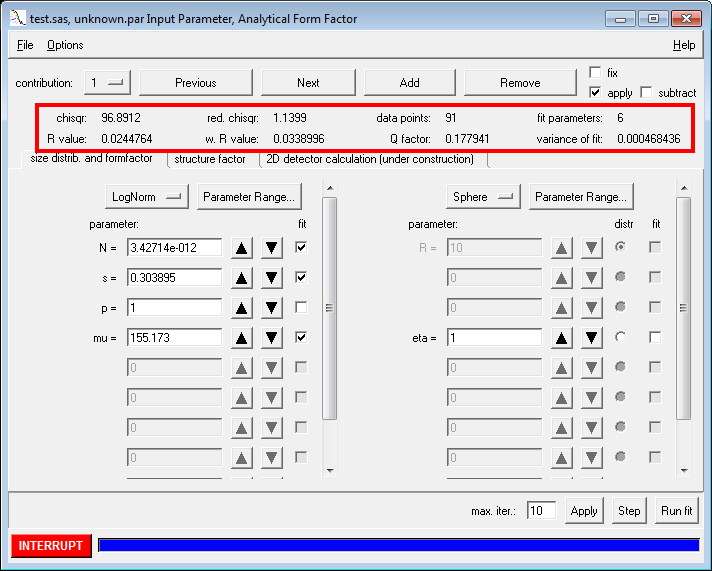
\includegraphics[width=0.712\textwidth]{../images/related_pages/goodnessOFfitPAR.png}
\end{center}
\caption{The parameters $Q, R,R_w$, describing the goodness of the fit, are displayed in the marked area of the GUI}
\label{fig:GoodnessParGUI}
\end{figure}

%~\\
\subsection{Confidence interval of the fitting parameter}
~\\

The confidence intervals of the fitting parameters are calculated at the minimum of the $\chi^2$. At the minimum first the partial derivatives according to the fit parameters $a_i$ are calculated to get the matrix elements $A_{kl}$ via
\begin{align}
A_{kl} &= \sum_{i=1}^{N} \frac{1}{\left(\Delta I_i^\mathrm{th}\right)^2} \frac{\partial I_i^\mathrm{th}(q_i,\mathbf{a})}{\partial a_k} \frac{\partial I_i^\mathrm{th}(q_i,\mathbf{a})}{\partial a_l}
\end{align}
The inversion of this matrix yield the covariance matrix
\begin{align}
        \mathbf{C} &= \mathbf{A}^{-1}
\end{align}
The standard deviations $\Delta a_i$ of the best-fit parameters are given by the square root of the corresponding diagonal elements of the covariance matrix
\begin{align}
\Delta a_i &= \sqrt{C_{ii}}
\end{align}
The correlation coefficient of the fit parameters $a_k$ and $a_l$ are given by
\begin{align}
r_{kl} &= \frac{C_{kl}}{\sqrt{C_{kk}C_{ll}}} = \frac{C_{kl}}{\Delta a_k \Delta a_l}
\end{align}
Both the non-diagonal elements of the correlation matrix $r_{k>l}$ and the confidence intervals of the fitting parameters $\Delta a_k$ are calculated when the fit converges and displayed in a GUI (fig.\ \ref{fig:ErrorGUI}) which can be opened via a menu button as shown in fig.\ \ref{fig:ErrorButton}.

\begin{figure}[htb]
\captionsetup[subfigure]{position=b}
\centering
\subcaptionbox{menu button showing the GUI for the confidence intervals and correlation matrix \label{fig:ErrorButton} }{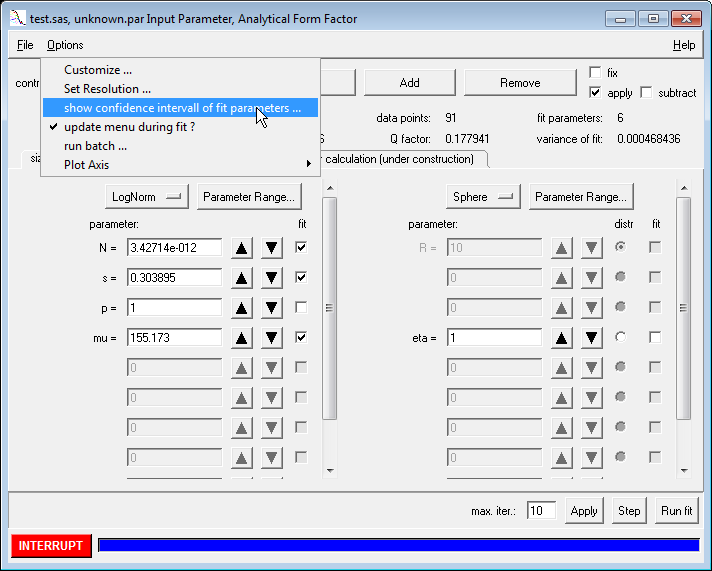
\includegraphics[width=0.47\textwidth]{../images/related_pages/menueConfidenceIntervall.png}}
\hfill
\subcaptionbox{GUI displaying the fitting parameters including confidence intervals and correlation matrix \label{fig:ErrorGUI} }{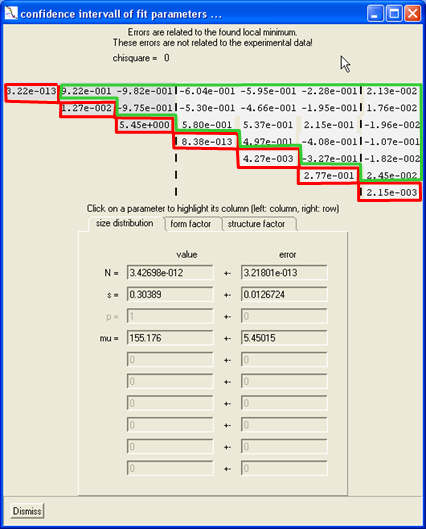
\includegraphics[width=0.47\textwidth]{../images/related_pages/ConfidenceIntervallANDCorrelationMatrix.png}}
\caption{The confidence intervals are calculated at the end of the minimization procedure.}
\label{fig:FitErrors}
\end{figure}

The routine can give nonphysical confidence intervals if
\begin{itemize}
\item no proper error bar for the experimental data are supplied
\item a wrong physical model for describing the data is used
\item the physical model has strongly correlated parameters
\begin{subequations}
\begin{align}
r_{kl} &\approx 0, a_k \mbox{ and } a_l \mbox{ are uncorrelated parameters} \\
r_{kl} &\approx \pm 1, a_k \mbox{ and } a_l \mbox{ are strongly correlated parameters}
\end{align}
\end{subequations}
\end{itemize}

The given value for the confidence interval of the fit parameters should not be used in the cases
\begin{itemize}
\item where the error is not normal distributed
\item where the data is given without error bar
\item where parameters are strongly correlated
\end{itemize}

\clearpage
\section{references to numerical strategies \SASfit make use of}

\subsection{integration or quadrature strategies} ~\\

In \SASfit several tasks require specialized integration routines. At the moment \SASfit supplies the function \texttt{sasfit\_integrate()}, \texttt{sasfit\_cubature()},
\texttt{sasfit\_orient\_avg()}, and \texttt{sasfit\_hankel()}.
\texttt{sasfit\_integrate()} performs one-dimensional integrations and \texttt{sasfit\_cubature()} multidimensional integrations over multi-dimensional cubes. \texttt{sasfit\_orient\_avg()} performs efficient integrations over the surface of a sphere to perform orientational averages. \texttt{sasfit\_hankel()} supplies highly optimized routines for Bessel or Hankel transforms containing oscillatory Bessel functions in the integrand. The window for fitting or simulating data (fig.\ \ref{fig:CustomizeIntGUI}) has a menu option under \texttt{[Options|Customize...]} opening a window to configure the internal integration routines.
\begin{figure}[htb]
\begin{center}
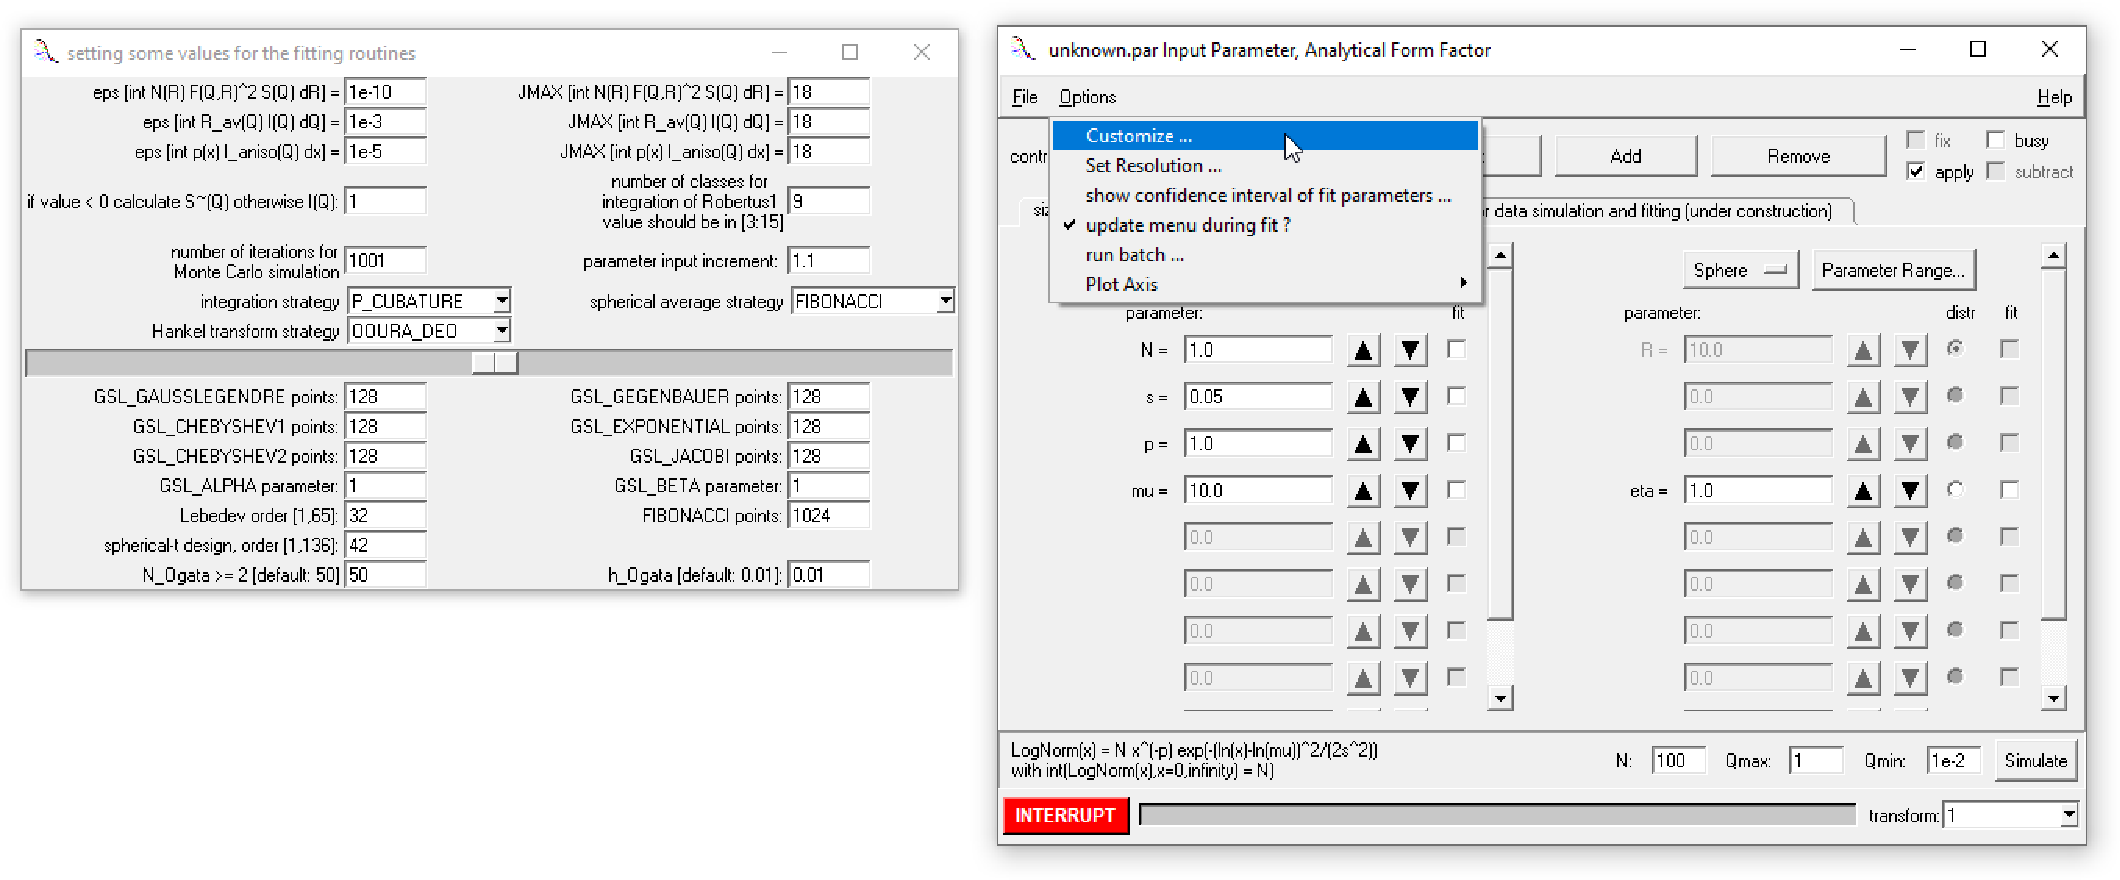
\includegraphics[width=0.95\textwidth]{../images/GUI/CustomizeWindow.pdf}
\end{center}
\caption{Menu for configuring internal integration routines in \SASfit}
\label{fig:CustomizeIntGUI}
\end{figure}

\texttt{sasfit\_integrate()}  and \texttt{sasfit\_cubature()} have the same configuration options. For multidimensional integrations either specialized algorithms or nested calls of one dimensional integration routines are used. Possible options for them are
\begin{description}
   \item[\texttt{OOURA\_DE}] This is an implementation of an double-exponential quadrature algorithm from \cite{Mori1990,Mori2001}
   \item[\texttt{OOURA\_CC}] Clenshaw-Curtis-Quadrature using Chebyshev Series Expansion (\url{https://www.kurims.kyoto-u.ac.jp/~ooura/intcc.html})
   \item[\texttt{TANHSINH\_1}] TanhSinh quadrature \cite{Engelen2021,Engelen}
   \item[\texttt{TANHSINH\_2}] TanhSinh quadrature \cite{Engelen2021,Engelena}
   \item[\texttt{GSL\_QUAD}] quad integration routine from gsl \cite{Galassi2021}
   \item[\texttt{GSL\_QAG}] QAQ integration routine from gsl \cite{Galassi2021}
   \item[\texttt{GSL\_QNQ}] QNQ integration routine from gsl \cite{Galassi2021}
   \item[\texttt{H\_CUBATURE}] multidimensional integration routine \texttt{hcubature} from \cite{Johnson2017}
   \item[\texttt{P\_CUBATURE}] multidimensional integration routine \texttt{pcubature} from \cite{Johnson2017}
   \item[\texttt{GSL\_LEGENDRE}] Gauss-Legendre quadrature using gsl library  \cite{Galassi2021}
   \item[\texttt{MC\_MISER}] Monte-Carlo integration algorithm Miser using gsl library  \cite{Galassi2021}
   \item[\texttt{MC\_VEGAS}]  Monte-Carlo integration algorithm Vegas using gsl library  \cite{Galassi2021}
   \item[\texttt{MC\_PLAIN}]  plain Monte-Carlo integration algorithm using gsl library  \cite{Galassi2021}
   \item[\texttt{QMC\_HOLTON}] quasi Monte Carlo integration \cite{Zaslavsky2023} using the \texttt{gsl\_qrng\_halton} quasi random number generator from gsl \cite{Galassi2021}.
   \item[\texttt{QMC\_REVERSEHALTON}] quasi Monte Carlo integration \cite{Zaslavsky2023} using the \texttt{gsl\_qrng\_reversehalton} quasi random number generator from gsl \cite{Galassi2021}.
   \item[\texttt{QMC\_SOBOL}] quasi Monte Carlo integration \cite{Zaslavsky2023} using the \texttt{gsl\_qrng\_sobol} quasi random number generator from gsl \cite{Galassi2021}.
   \item[\texttt{QMC\_NIEDERREITER\_2}] quasi Monte Carlo integration \cite{Zaslavsky2023} using the reverse \texttt{gsl\_qrng\_niederreiter\_2} quasi random number generator from gsl \cite{Galassi2021}.
   \item[\texttt{RQMC\_SOBOL\_RDS}] randomized quasi Monte Carlo integration using the quasi random Sobol sequence with additional random digit scrambling \cite{Burley2020Scrambling}
   \item[\texttt{RQMC\_SOBOL\_OWEN}] randomized quasi Monte Carlo integration using the quasi random using Owen-scrambled Sobol sequence \cite{Burley2020Scrambling,Owen1995}
   \item[\texttt{RQMC\_FAURE05}] randomized quasi Monte Carlo integration using Owen-scrambled Faure (0,5) sequence \cite{Burley2020Scrambling,Owen1995}.
   \item[\texttt{RQMC\_LAINE\_KARRAS}] randomized quasi Monte Carlo integration using Laine-Karras hash method mentioned in \cite{Burley2020Scrambling} and given as C source code in its supplement information.
\end{description}

\texttt{sasfit\_orient\_avg()}
\begin{description}
\item[\texttt{GSL\_2D\_GAUSSLEGENDRE}]
\item[\texttt{Lebedev}]
\item[\texttt{FIBONACCI}]
\item[\texttt{HCUBATURE}]
\item[\texttt{PCUBATURE}]
\item[\texttt{spherical\_t\_design}]
\item[\texttt{OOURA\_DE}]
\item[\texttt{OOURA\_CC}]
\item[\texttt{GSL\_CQUAD}]
\item[\texttt{TANHSINH\_1}]
\item[\texttt{TANHSINH\_2}]
\item[\texttt{MC\_VEGAS}]
\item[\texttt{MC\_MISER}]
\item[\texttt{MC\_PLAIN}]
\item[\texttt{QMC\_NIEDERREITER\_2}]
\item[\texttt{QMC\_SOBOL}]
\item[\texttt{QMC\_HALTON}]
\item[\texttt{QMC\_REVERSEHALTON}]
\item[\texttt{RQMC\_SOBOL\_RDS}]
\item[\texttt{RQMC\_SOBOL\_OWEN}]
\item[\texttt{RQMC\_FAURE05\_OWEN}]
\item[\texttt{RQMC\_LAINE\_KARRAS}]
\end{description}

 \texttt{sasfit\_hankel()} \cite{Chave1983,Anderson1989,Ooura_1991,Guptasarma1997,Ogata2005,Kong2007,Key2012,Kang2021}
\begin{description} 
\item[\texttt{OOURA\_DEO}]
\item[\texttt{OGATA\_2005}]
\item[\texttt{FBT0}]
\item[\texttt{FBT1}]
\item[\texttt{FBT2}]
\item[\texttt{GSL\_QAWF}]
\item[\texttt{GUPTASARMA\_97}]
\item[\texttt{GUPTASARMA\_97\_FAST}]
\item[\texttt{KEY\_51}]
\item[\texttt{KEY\_101}]
\item[\texttt{KEY\_201}]
\item[\texttt{ANDERSON\_801}]
\item[\texttt{QWE}]
\item[\texttt{CHAVE}]
\end{description}

\clearpage
\section{Fitting strategies}
